\chapter{Ejercicio aspiradora robótica atrapa confeti}\label{chap:aspiradora}
En los siguientes capítulos se explica el proceso de desarrollo de los tres ejercicios realizados en este trabajo fin de grado. Este capítulo está dedicado al primero de ellos, este ejercicio consiste en una aspiradora robótica que atrapa piezas de confeti dispersas por el suelo de una casa. En primer lugar se expone el enunciado y los objetivos. En segundo lugar cómo se ha implementado y creado los modelos de robot aspiradora y escenario para la plataforma Kibotics. Finalmente se muestran las soluciones de referencia creadas en Python y Scratch que satisfacen el objetivo del ejercicio.

Para hacer el ejercicio descrito a continuación, se utilizaron las herramientas Blender, el simulador Websim de Kibotics que contiene la tecnología A-Frame y los lenguajes JavaScript, HTML5 y JSON.

\section{Enunciado}
La finalidad de este ejercicio es programar una aspiradora robótica que se encuentre en una habitación y que ésta sea capaz de recoger piezas de confeti cuando pase por encima. El evaluador automático que se va a realizar nos servirá para contar el confeti recogido en un tiempo determinado.

El alumno deberá programar en Scratch o en Python un algoritmo de planificación de ruta para que consiga atrapar el mayor número de trozos de confeti en 5 minutos.

Para la visualización de este ejercicio y que los usuarios de Kibotics puedan acceder a él, se ha creado una página web. Gracias a esta página web, los usuarios tienen acceso a la teoría del ejercicio y  disponen de un editor y el simulador Websim necesarios para hacer el ejercicio. 

Se creó la teoría del ejercicio en HTML5 y se modificaron las plantillas que utiliza el servidor Django de Kibotics. El objetivo del usuario  es hacer un algoritmo de planificación de ruta utilizando los sensores y actuadores del robot para que cuando detecte un objeto próximo, por ejemplo una pared o una mesa, se mueva en ángulos aleatorios. 
En las siguientes figuras podemos ver la página de teoría donde se explica el objetivo del ejercicio, los requisitos (Figura 4.1), para explicar al alumno los diferentes algoritmos de cobertura que puede utilizar los aspiradores robóticos se ha añadido un poco de teoría (Figura  4.2), unas pequeñas pistas y un ``¿Sabías que... ? '' (Figura 4.3) hablando de las primeras aspiradoras y cómo funcionaban. 
\\

\begin{figure}[H]
    \centering
    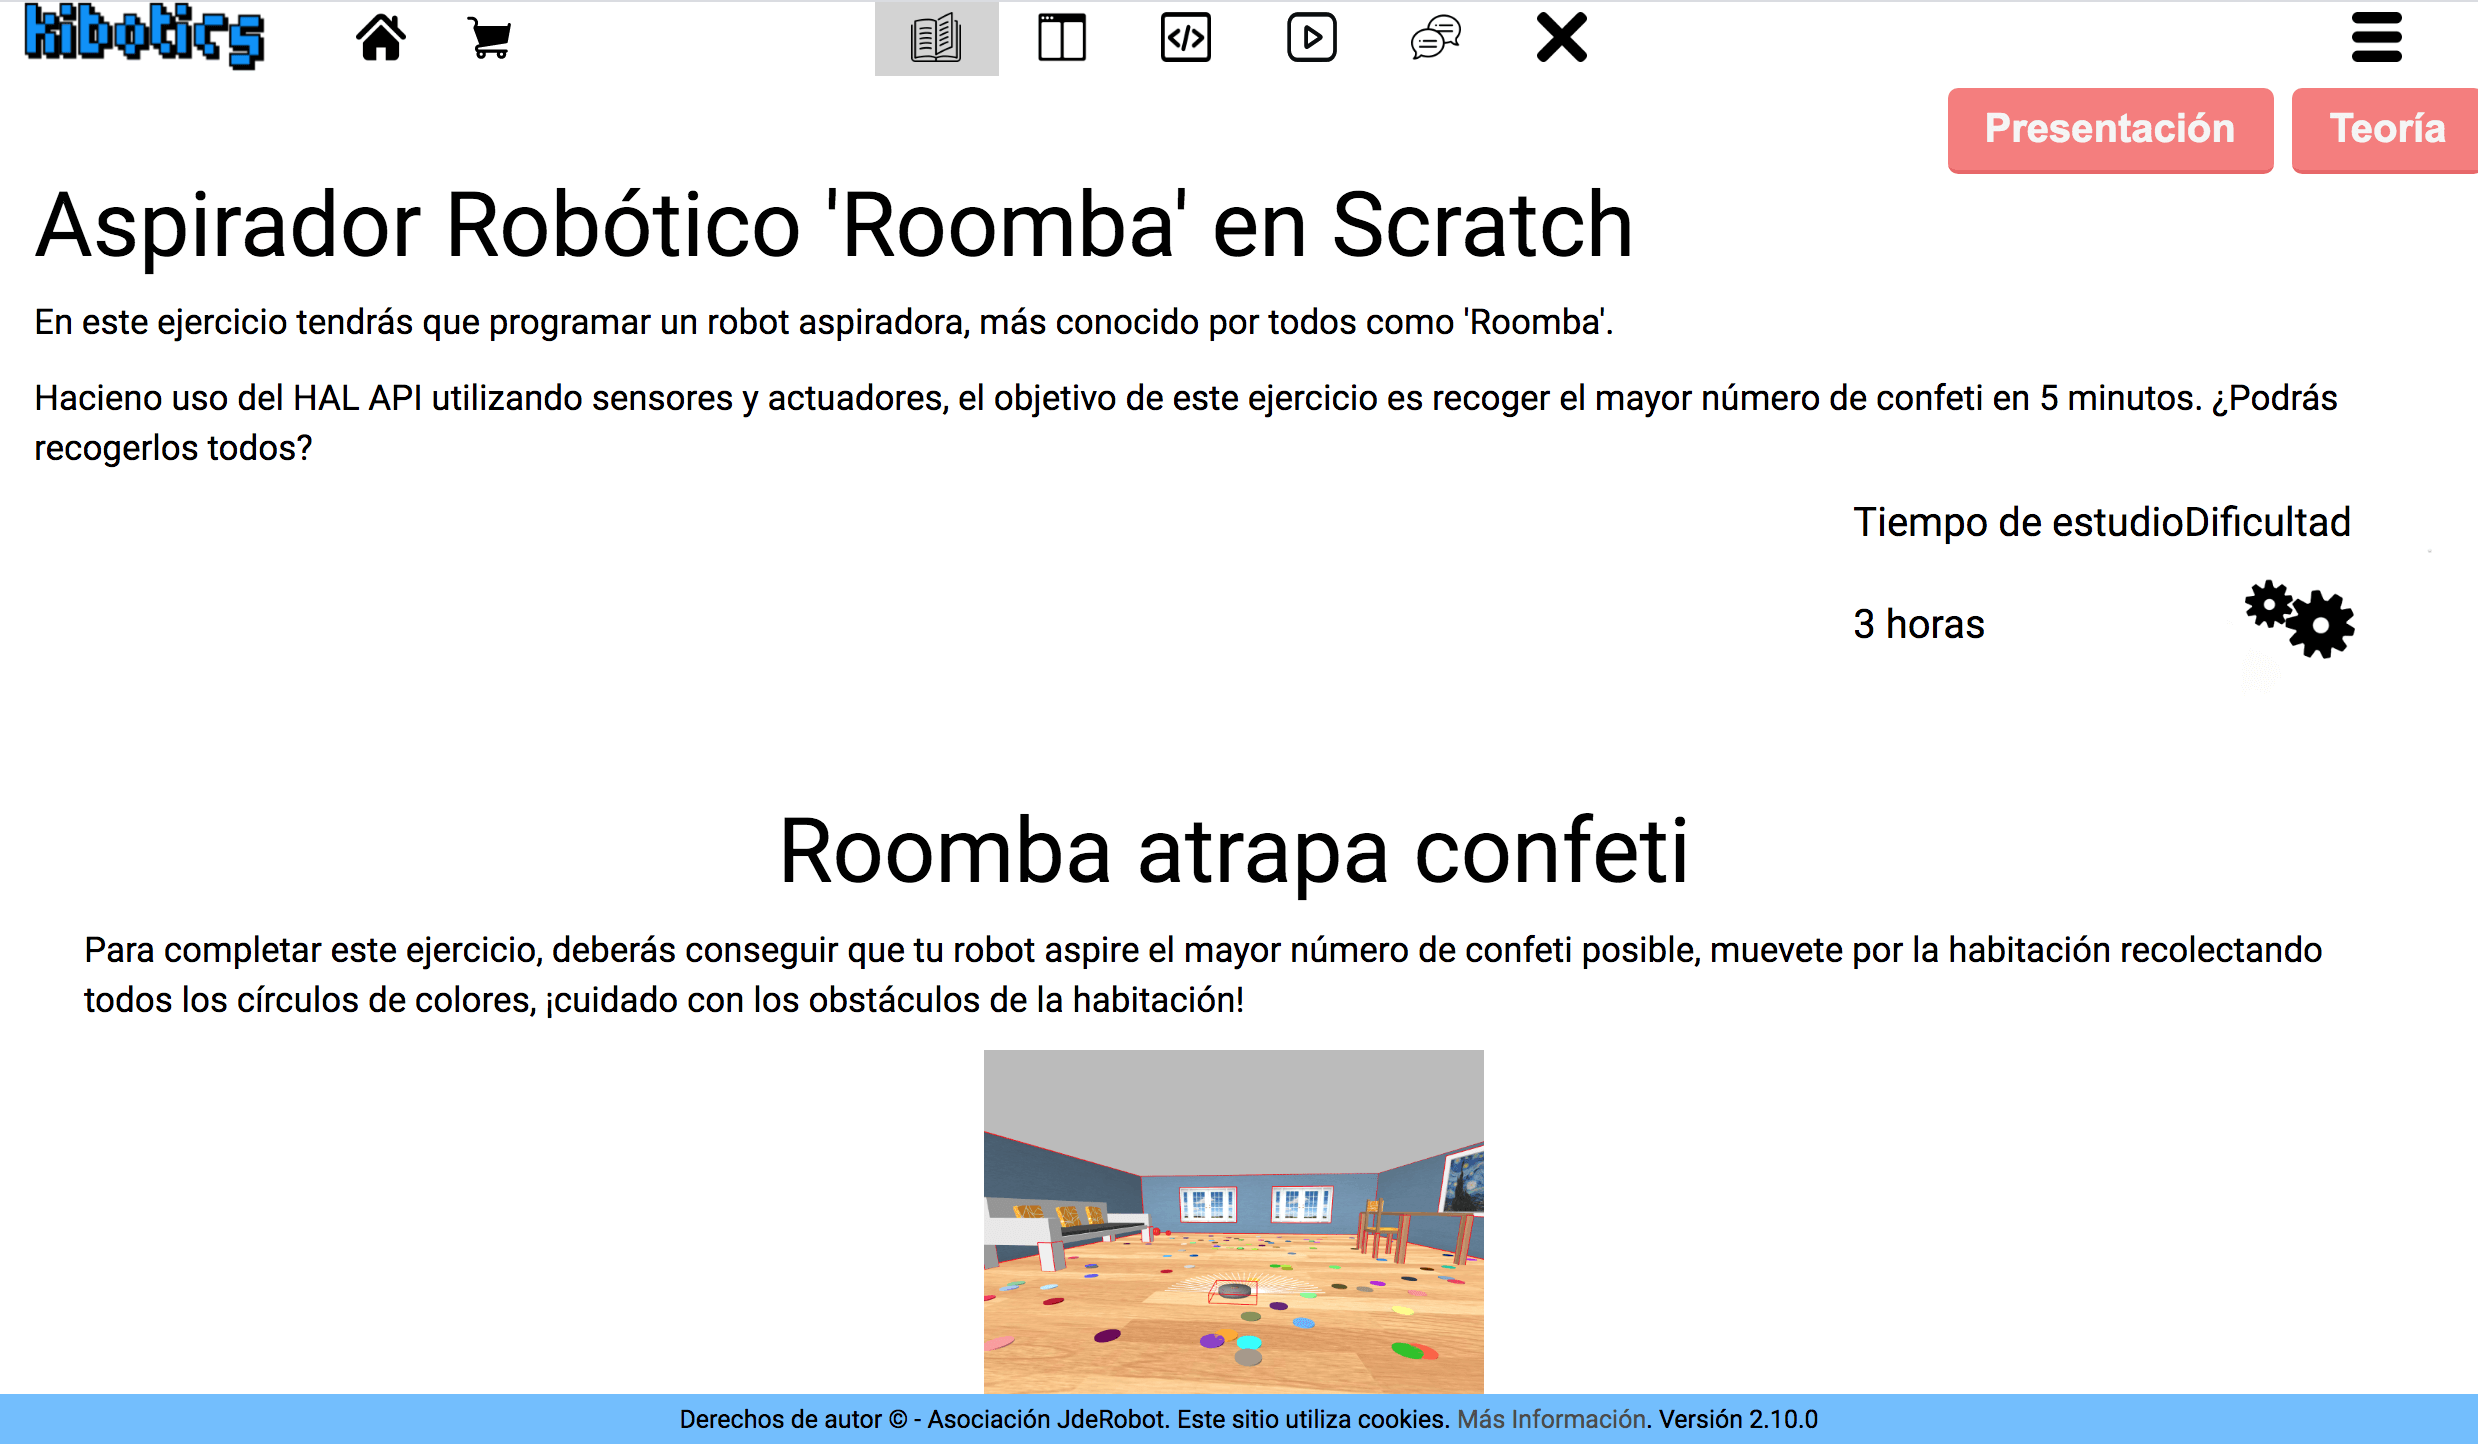
\includegraphics[width=1\textwidth, height=0.5\textwidth]{chapters/images/teoria1.png}
    \caption{Página de teoría enunciado y requisitos}
    \label{fig:my_label}
\end{figure}
\begin{figure}[H]
    \centering
    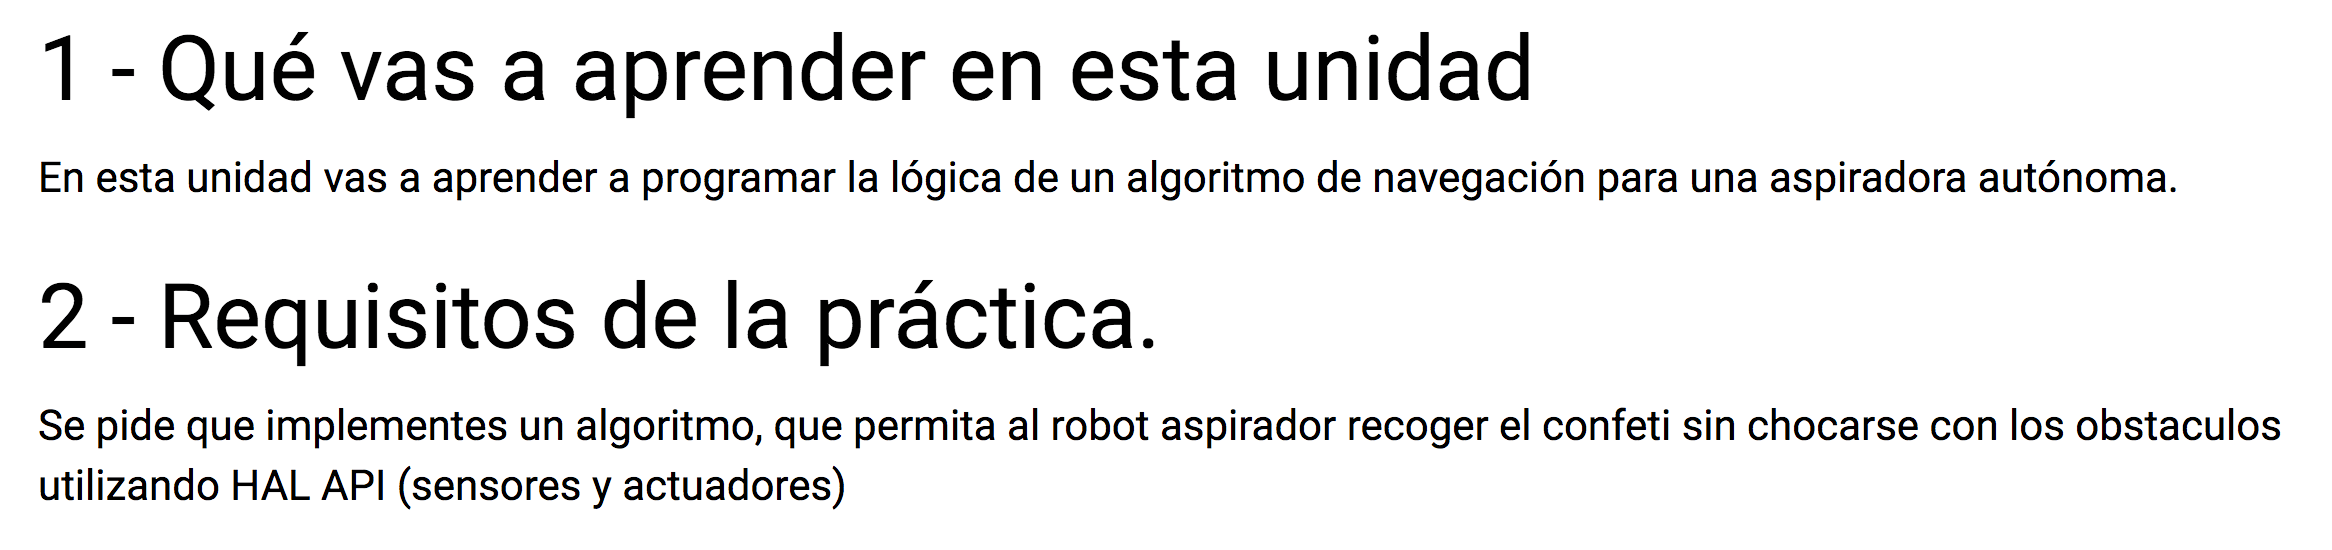
\includegraphics[width=1\textwidth, height=0.5\textwidth]{chapters/images/teoria2.png}
    \caption{Teoría}
    \label{fig:my_label}
\end{figure}
\begin{figure}[H]
    \centering
    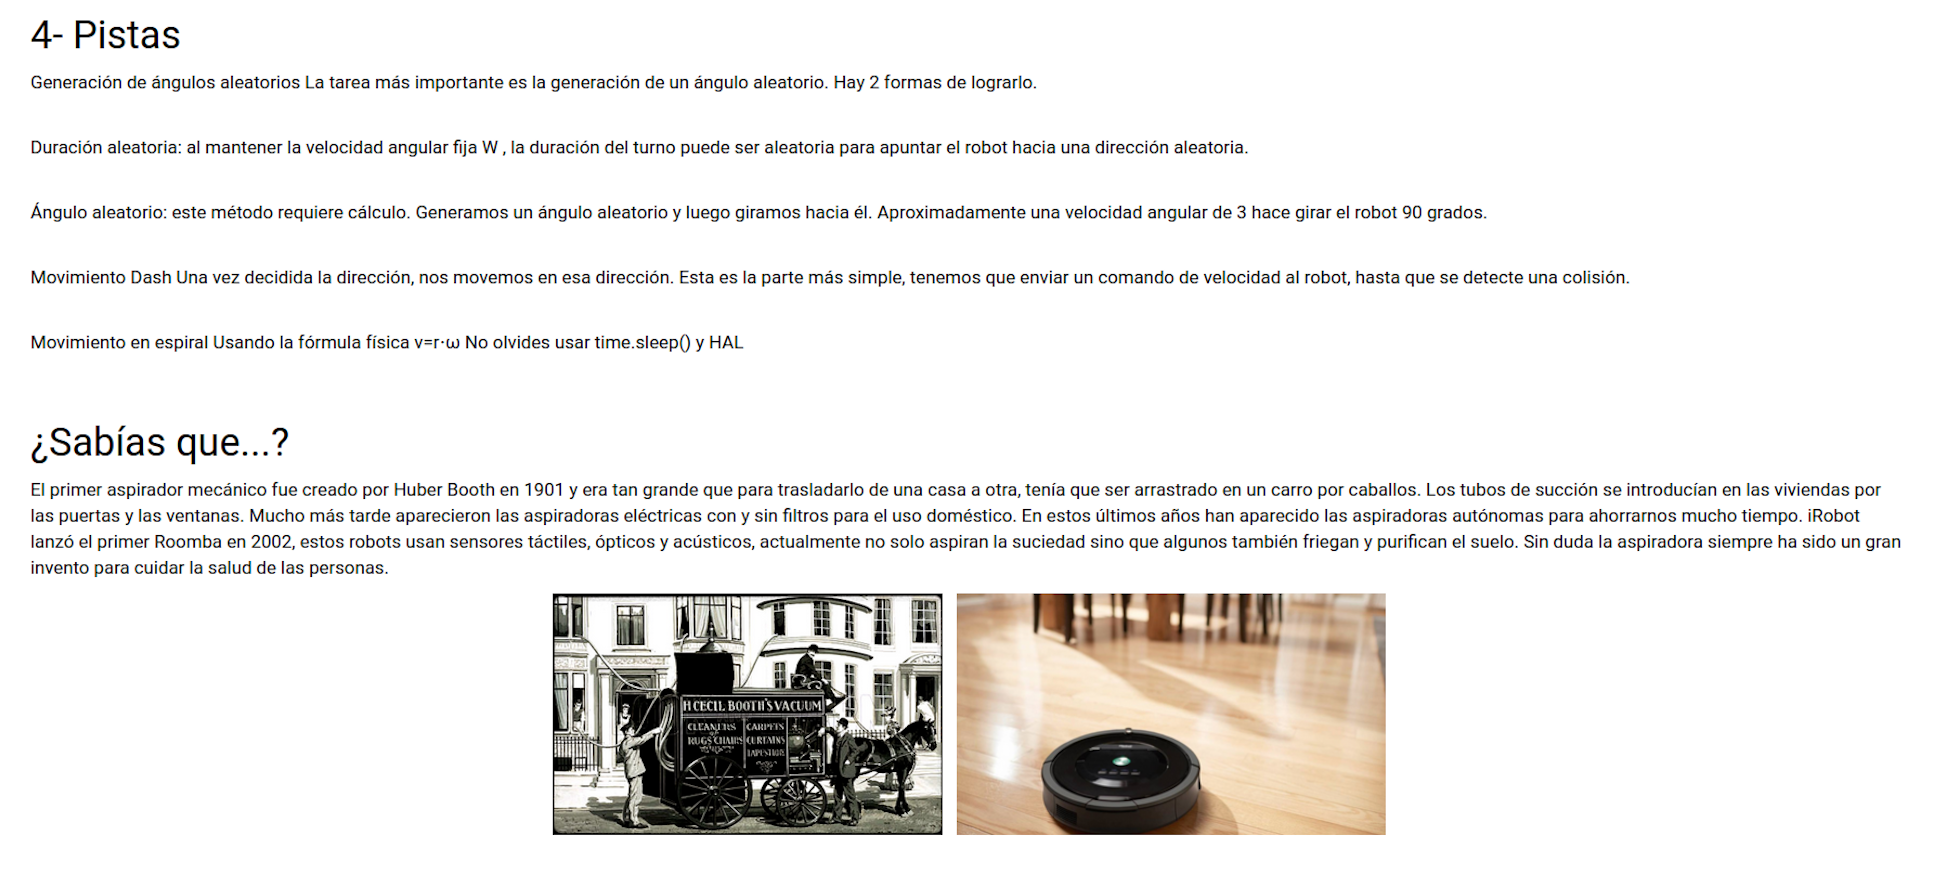
\includegraphics[width=1\textwidth, height=0.5\textwidth]{chapters/images/teoria3.png}
    \caption{Pistas y ¿sabías que.. ?}
    \label{fig:my_label}
\end{figure}

\section{Modelos del mundo}
Para este ejercicio se crearon nuevos muebles con Blender (ver Figuras 4.4 y 4.5) para que el escenario pareciera una habitación realista (ver Figura 4.6).
\begin{figure}[H]
  \begin{subfigure}[b]{0.5\textwidth}
  \centering
    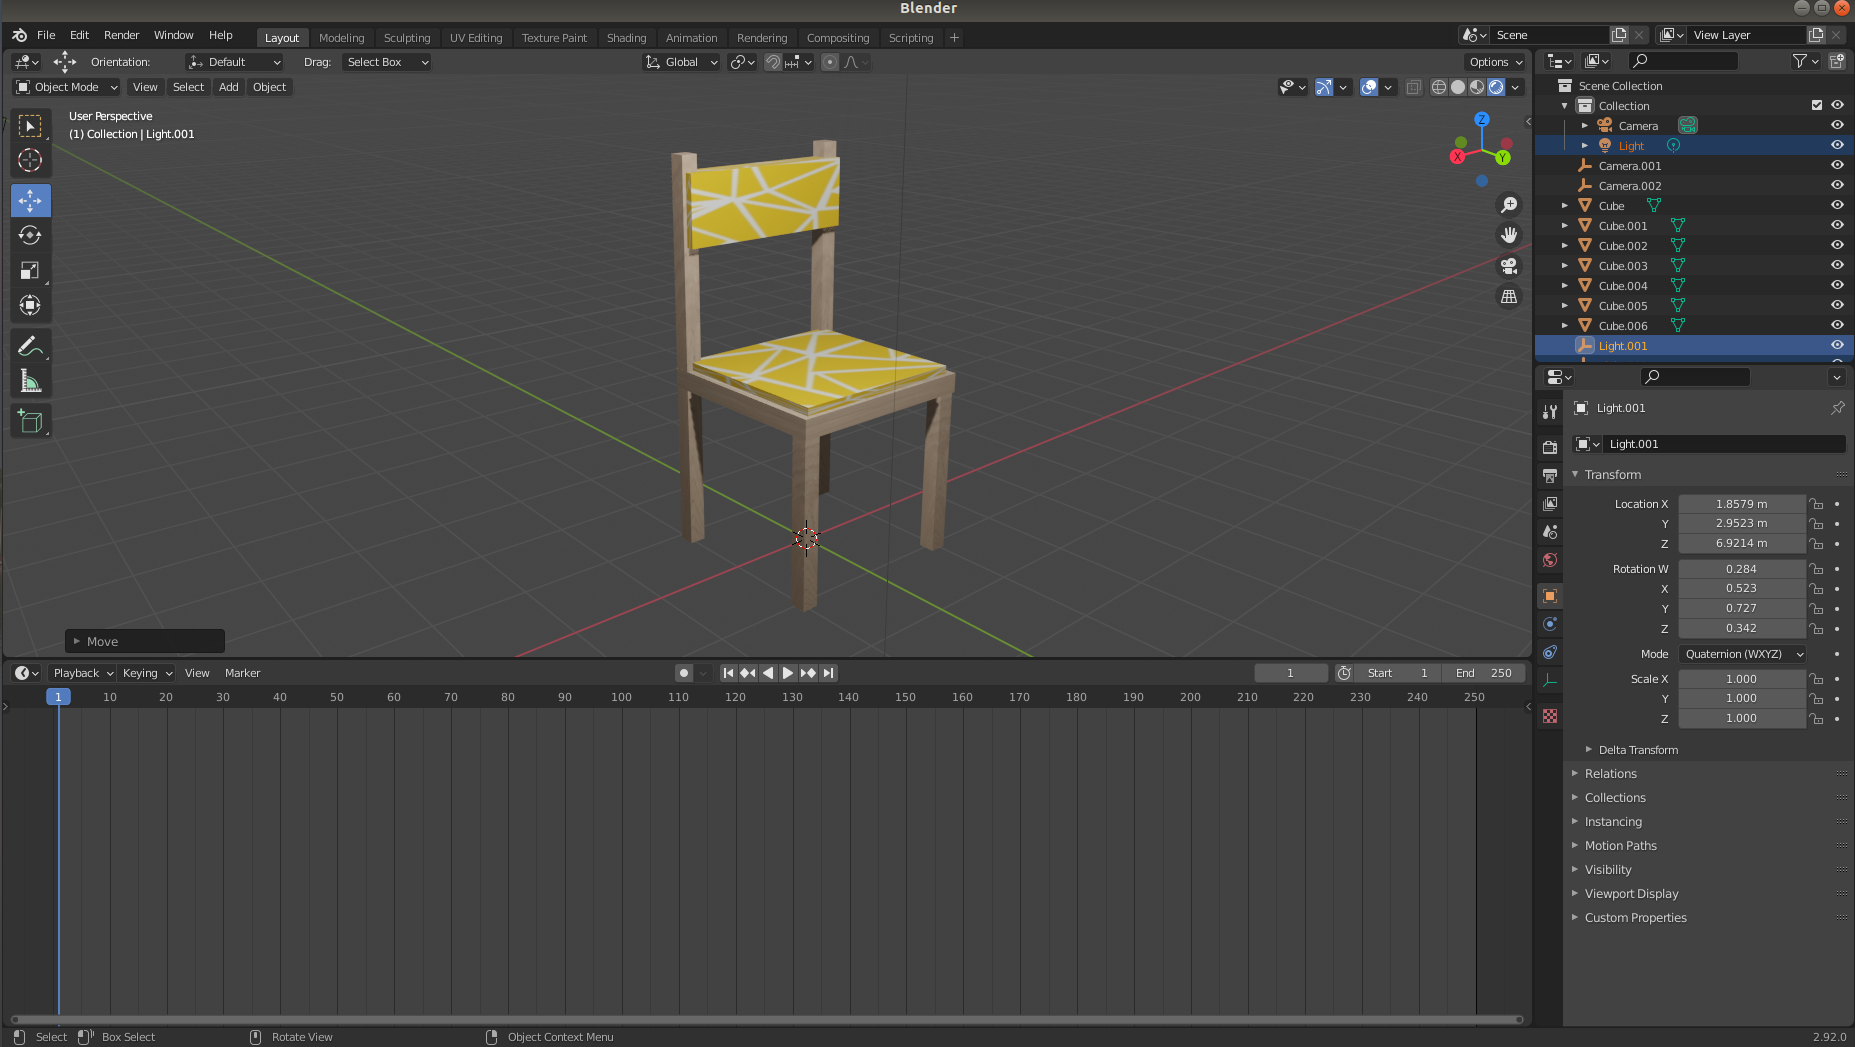
\includegraphics[width=0.95\textwidth, height=0.6\textwidth]{chapters/images/silla.png}
    \caption{Modelo silla}
    \label{fig:f1}
  \end{subfigure}
  \hfill
  \begin{subfigure}[b]{0.5\textwidth}
  \centering
    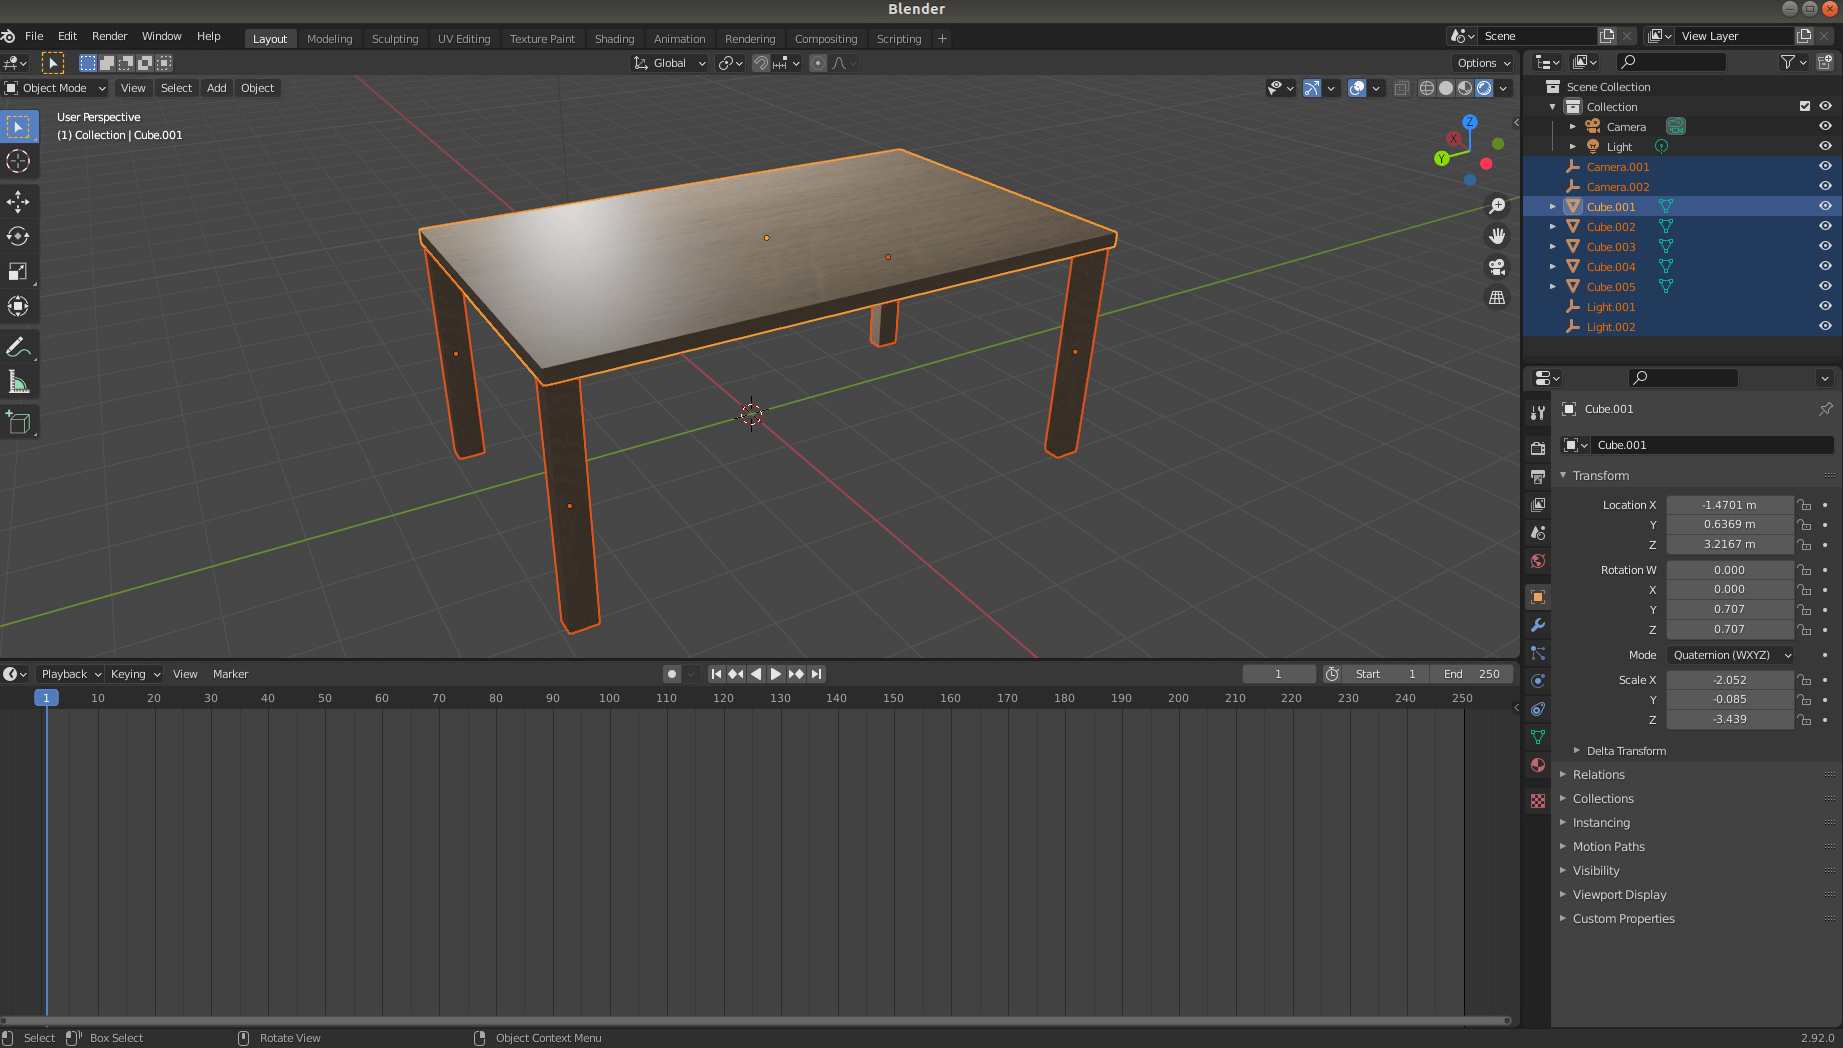
\includegraphics[width=0.95\textwidth, height=0.6\textwidth]{chapters/images/mesa.png}
	\caption{Modelo mesa}    
    \label{fig:f2}
 
  \end{subfigure}
  \caption{Modelos en Blender}
\end{figure}

\begin{figure}[H]
  \centering
 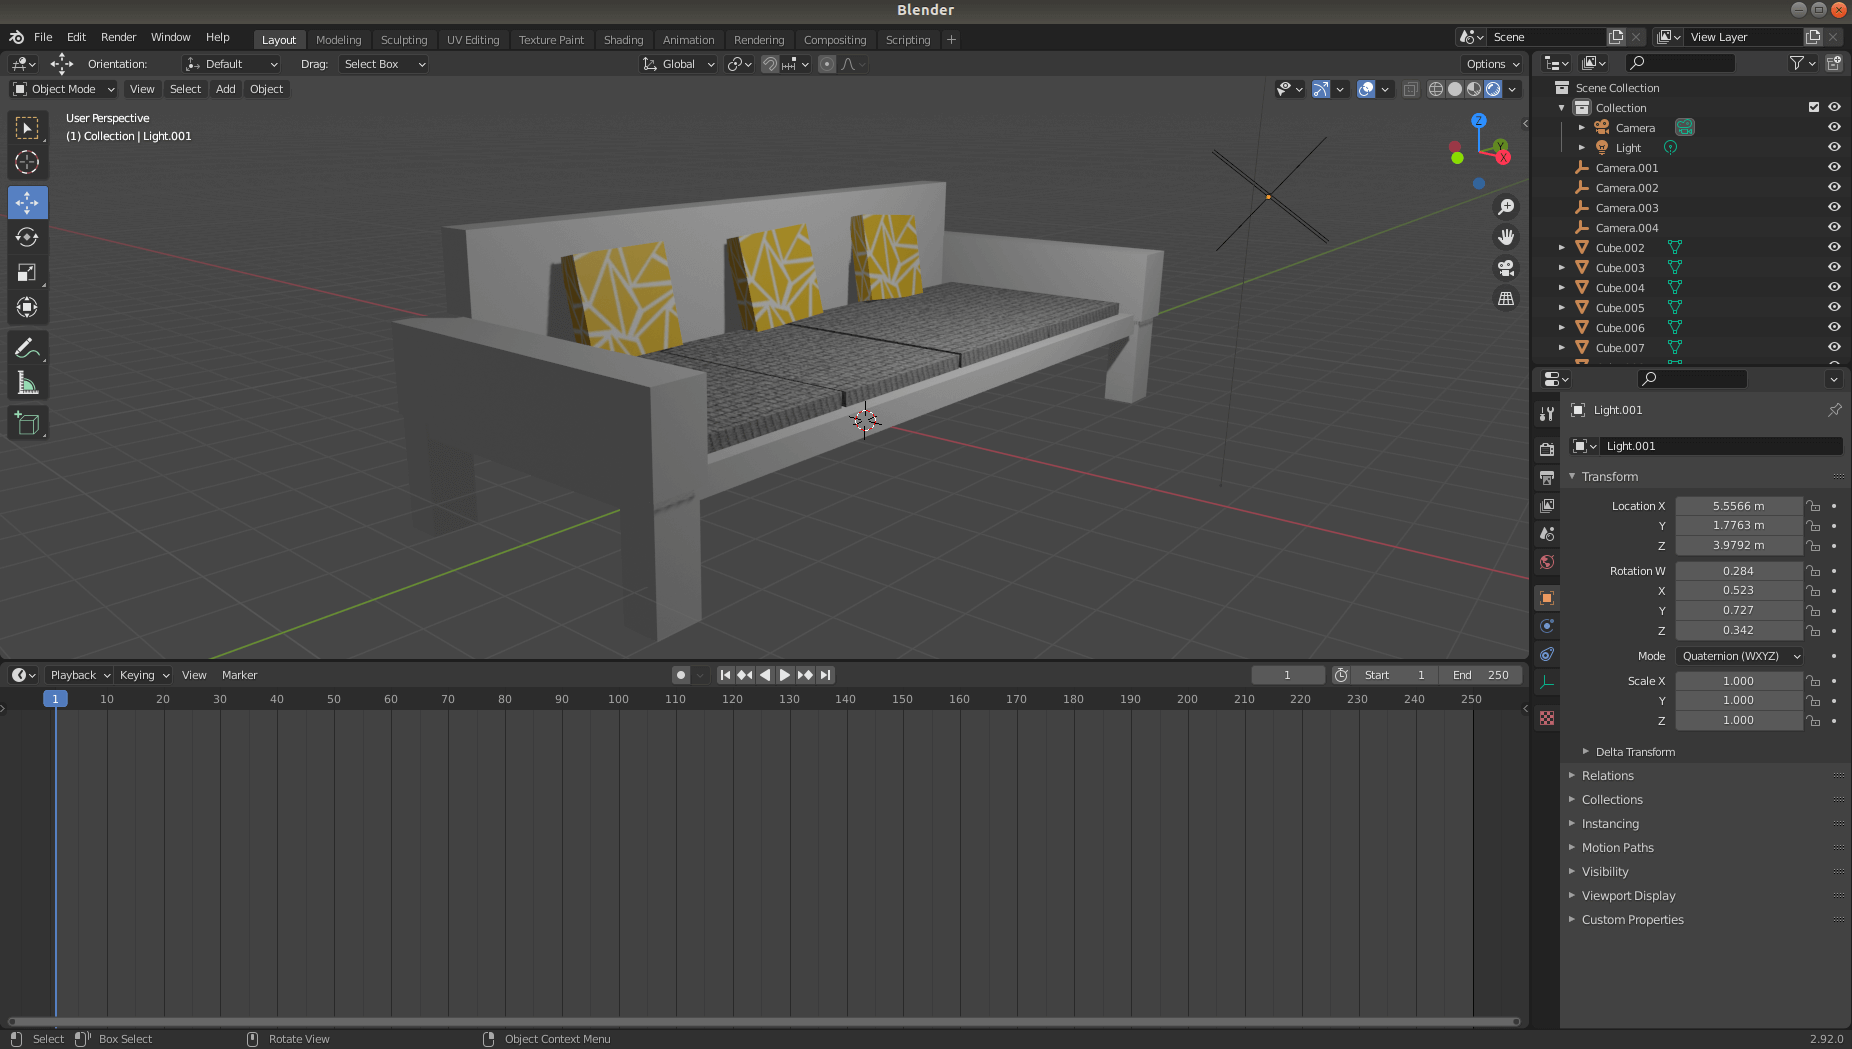
\includegraphics[width=0.7\textwidth]{chapters/images/sofa.png}
  \caption{Modelo sofá en Blender}
\end{figure}

\begin{figure}[H]
\centering
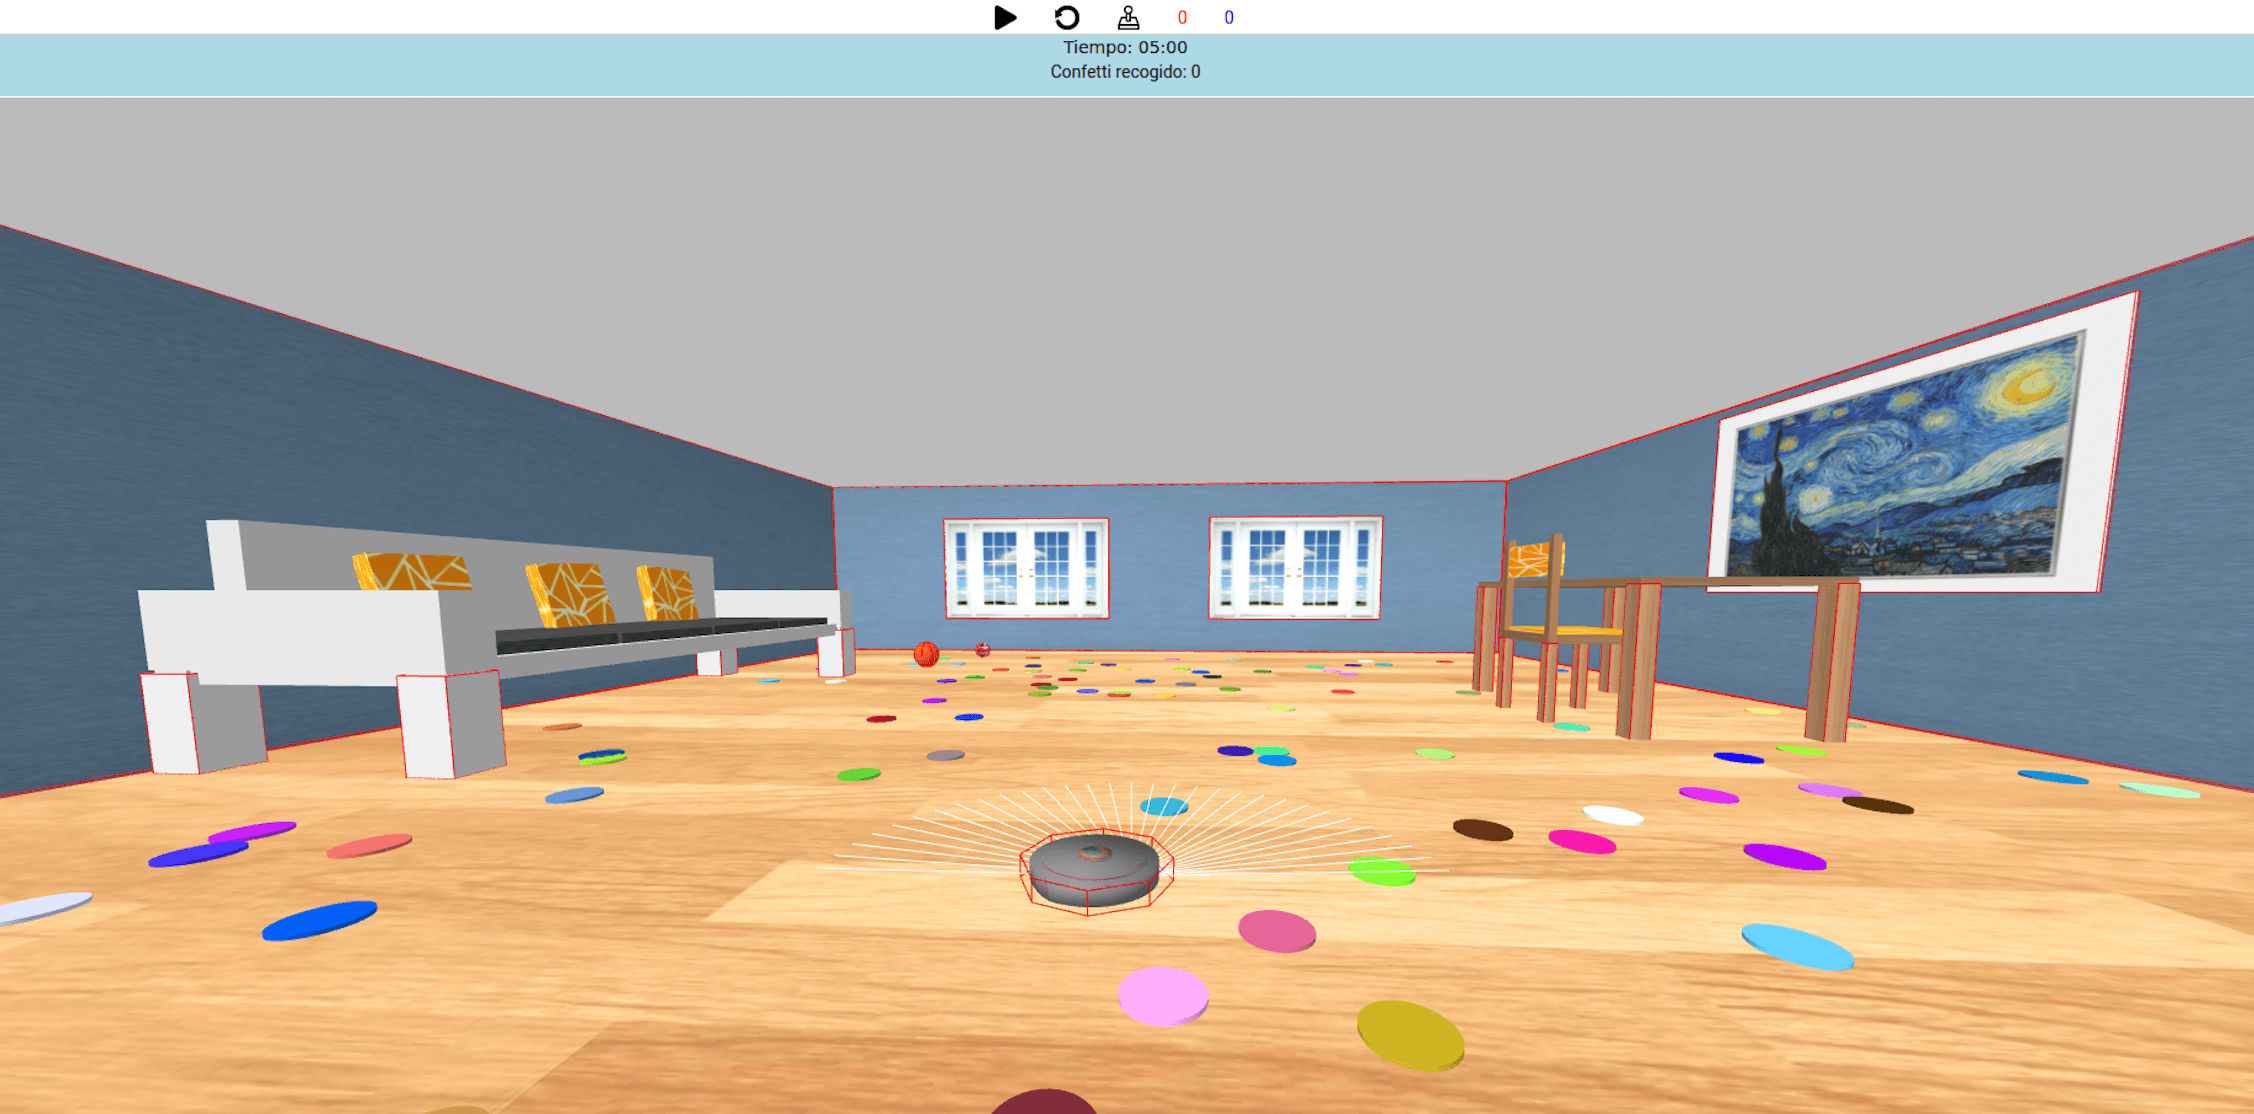
\includegraphics[width=0.8\textwidth, height=0.4\textwidth]{chapters/images/habitacioncon.png}
\caption{Habitación amueblada}
\end{figure}

Estos objetos se añadieron en el fichero de configuración json del ejercicio definiendo su identificador, modelo 3d gltf, la posición y la escala. El código que se muestra a continuación pertenece a la creación de la mesa pero  la estructura  de todos los elementos añadidos es la misma: 
\begin{lstlisting}
{
          "tag": "a-entity",
          "attr": {
              "id": "model-table",
              "gltf-model":"/static/websim/assets/models/mesa.gltf",
              "position":{"x":40, "y":0,"z":0},
              "scale": {"x":3,"y":3,"z":3}

          }
      },
\end{lstlisting}

También añadieron a ese fichero de configuración de una forma muy similar, las paredes, una puerta y un cuadro ajustando la posición, dimensiones y texturas correspondientes a cada uno.

Para que el ejercicio tenga mayor dificultad se introdujeron 2 pelotas con movimiento. Para conseguir este movimiento había dos posibilidades: animación desde Blender o Animación desde A-Frame. 
En el vídeo \footnote{https://www.youtube.com/watch?v=1JPb3Mw8638}  se puede ver cómo hacer una animación no lineal sencilla en Blender. Para poder usar animaciones de Blender en Websim es necesario que sean animaciones no lineales. Estudiando ambas opciones, se optó por la animación en A-Frame desde el fichero de configuración, que era el método ideal para Websim. De esta forma dejamos toda la creación de las pelotas, asignación de texturas, posición y  animación definido en la configuración.

Para animar un objeto desde A-Frame añadimos el atributo \textit{``animation"} y completamos los valores que sean necesarios como desde dónde a dónde quieres que se mueva  el objeto o el tiempo que quieres que tarde en hacer esa animación. Las dos pelotas tienen estos atributos con sus respectivos valores. Por ejemplo en el siguiente código se puede ver cómo se define la animación en diagonal de la pelota de baloncesto: 
\begin{lstlisting}
  {
            "tag": "a-sphere",
            "attr": {
                "id":"basketball",
                "position": { "x":-40, "y":1.5, "z":-40 },
                "rotation": { "x":0, "y":0, "z":0 },
                "radius": 1.5,
                "src":"#basketball",
                "static-body": {
                    "mass": 2
                },              
	           "class":"collidable",
                "animation": "property: position; from: -40 1.5 -40 ;to: 40 1.5 40; dir: alternate; dur: 10000; loop: true"

            }
        },

\end{lstlisting}

En el escenario de este ejercicio habrá un conjunto de 100 trozos de papel, confeti, repartidos por el suelo. El modelo de confeti se va a crear con la etiqueta \textit{a-cylinder} de A-Frame. 

El confeti no se crea desde el fichero de configuración dado que se tendrían que crear uno a uno  todos los confetis y se extendería demasiado el fichero. Lo que se ha hecho es que, una vez esta cargado el mundo en el navegador del usuario, usando JavaScript, creamos dinámicamente todos los confetis.

Primero se generó un programa para fijar aleatoriamente las posiciones de los confetis en el mundo, así los confetis quedan esparcidos por la habitación y todos los alumnos cuentan con el mismo escenario. Estas posiciones x, y, z de los confetis se guardaron en otro fichero JSON llamado \textit{data.json}. En total el escenario está formado por 100 confetis de colores. El color de cada confeti se elige aleatoriamente cuando se crea desde JavaScript .

Parte del fichero data.json: 
\begin{lstlisting}
  data = '[{"x":-39,"y":0,"z":-14},
                {"x":7,"y":0,"z":-11},
                {"x":-6,"y":0,"z":-9},
                {"x":-33,"y":0,"z":28},
                {"x":-11,"y":0,"z":41},
                {"x":-11,"y":0,"z":-13},
                {"x":19,"y":0,"z":23},
                {"x":19,"y":0,"z":-30},
                {"x":-4,"y":0,"z":-27},
                {"x":25,"y":0,"z":20},
                ....]'
 \end{lstlisting}


Para leer el fichero \textit{data.json} se utiliza esté código en la plantilla HTML del ejercicio.
\begin{lstlisting}
 <script type="text/javascript" src="{\% static '/data.json' \%}"></script > 
 \end{lstlisting}


En el siguiente código podemos ver cómo se crea el confeti con la función \textit{document.createElement(`a\- cylinder')}. Una vez creado se le asignan los atributos con la función  \textit{setAttribute}.  El identificador es confeti más un número  n, n es un número de 0-99 que se le asigna para crear 100 confetis diferentes (ejemplo de id del confeti número 50   id=``confeti50"). Además se le asigna los atributos posición, con la posición correspondiente que se lee del \textit{data.json}, el color que es  aleatorio, como es un cilindro, se define la altura y radio del confeti.
Los confetis no cuentan con malla de colisión para que el aspirador pueda pasar por encima de ellos y absorberlos de una forma más natural.
Estas son las funciones necesarias para la creación de las piezas de confeti: 
\begin{lstlisting}

function getRandomColor() {
    var letters = '0123456789ABCDEF';
    var color = '#';
    for (var i = 0; i < 6; i++) {
      color += letters[Math.floor(Math.random() * 16)];
    }
    return color;
}

document.addEventListener('robot-loaded', (evt)=>{
    localRobot = evt.detail;
    console.log(localRobot);

    var sceneEl = document.querySelector('a-scene');

    // CREATE CONFETI
    var n = 0;
    var n_confetis = 99;
    score = 0;
    var array = JSON.parse(data);

    for ( n = 0; n <=n_confetis ; n++) {
      var c = document.createElement('a-cylinder');
      var num_conf="confeti"+ String(n)
      c.setAttribute('id', num_conf);
      pos = {x:array[n].x, y:0,z:array[n].z}
    
      c.setAttribute('position',pos);
    
      var color = getRandomColor();
      c.setAttribute('color', color);
      c.setAttribute('height', "0.25");
      c.setAttribute('radius', 1);
      sceneEl.appendChild(c);
}
\end{lstlisting}

\section{Modelo aspiradora}

El robot  propuesto en este ejercicio es una aspiradora robótica. Se crearon varios prototipos en Blender  hasta que se llegó al modelo final que podemos ver en la Figura 4.7. Su diseño está inspirado en los aspiradores robóticos más conocidos como Roomba o Dyson. El logo que aporta color al aspirador pertenece a la asociación JdeRobot \footnote{https://jderobot.github.io/}, pilar fundamental en el desarrollo de la plataforma Kibotics.
 
 \begin{figure}[H]
  \begin{subfigure}[b]{0.5\textwidth}
  \centering
    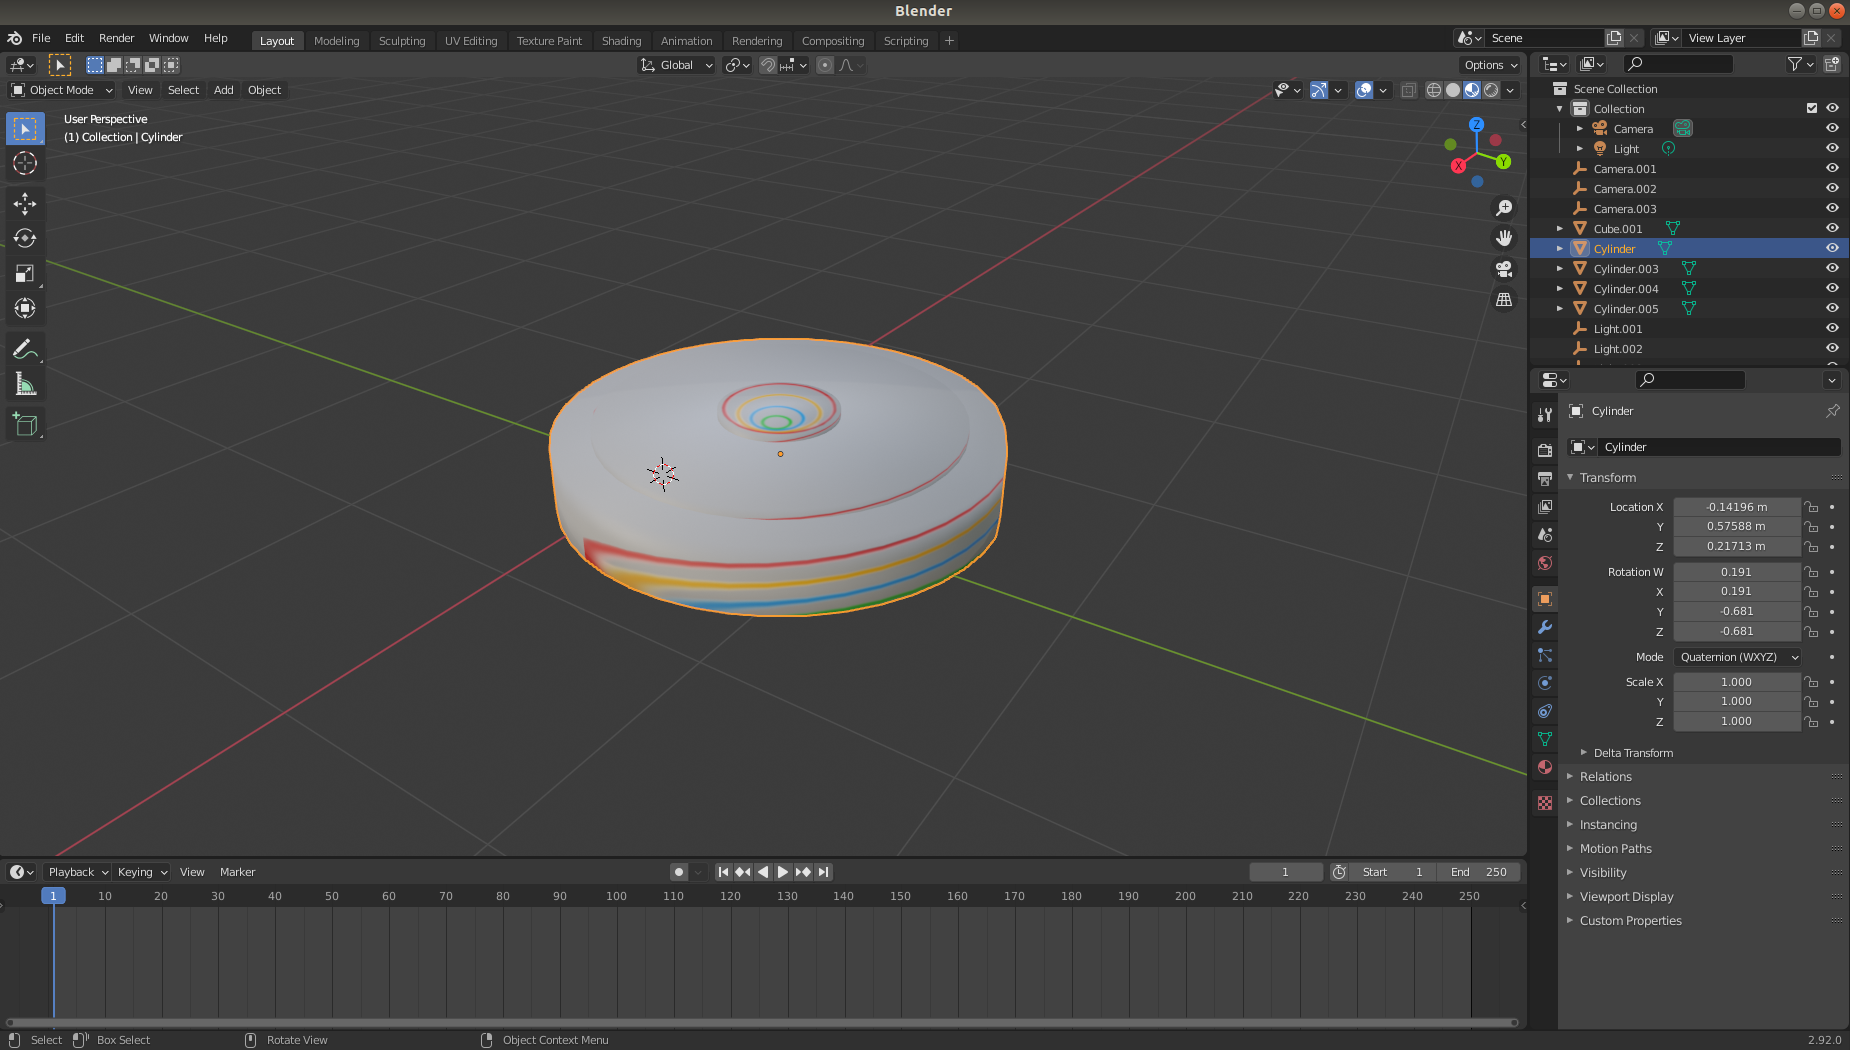
\includegraphics[width=0.95\textwidth, height=0.7\textwidth]{chapters/images/roombablender.png}
    \caption{}
    \label{fig:f1}
  \end{subfigure}
  \hfill
  \begin{subfigure}[b]{0.5\textwidth}
  \centering
    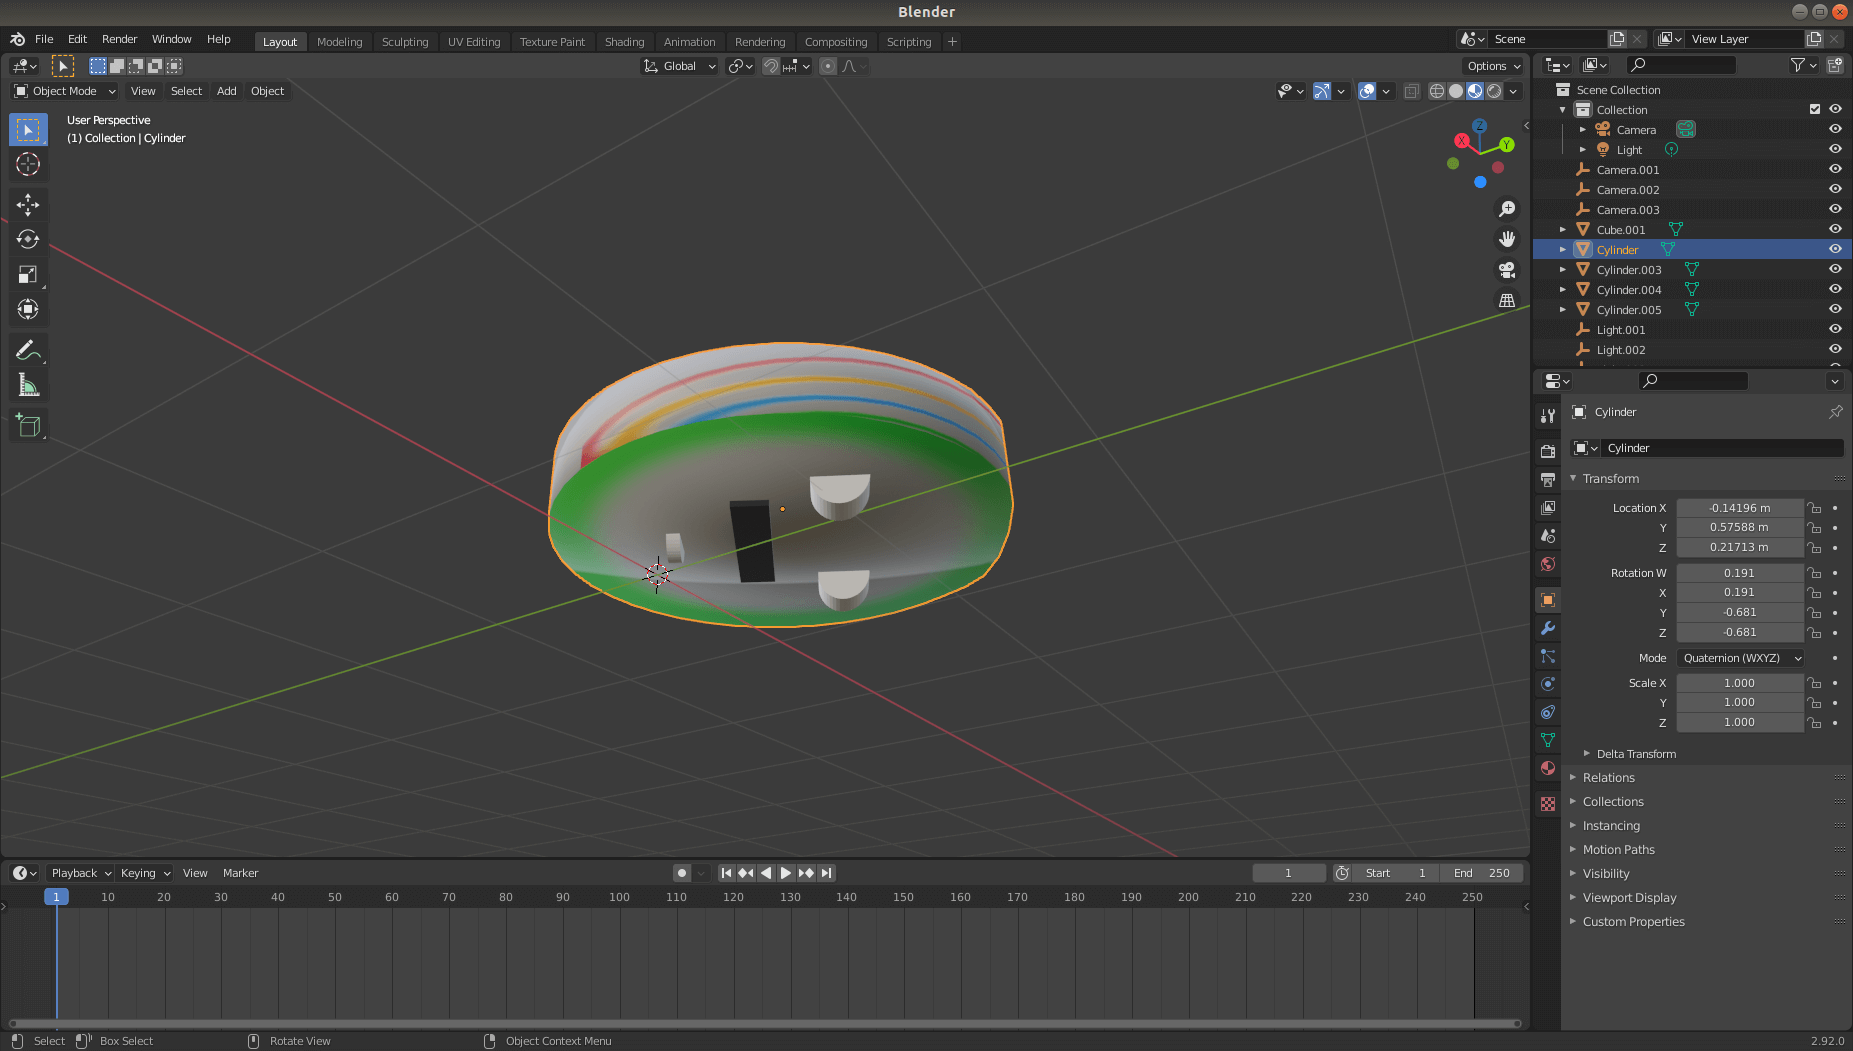
\includegraphics[width=0.95\textwidth, height=0.7\textwidth]{chapters/images/roombablender2.png}
	\caption{}    
    \label{fig:f2}
 
  \end{subfigure}
  \caption{Modelo de la aspiradora robótica  realizado en Blender.}
\end{figure}

Los robots en A-Frame está definidos por una apariencia 3D (geometría más texturas) y una malla de colisión.
El simulador Websim analiza ficheros JSON para formar mundos con la tecnología A-Frame. De esta forma es sencillo crear los objetos con pares \textit{``atributo": ``valor''}. A continuación podemos ver cómo se define el identificador robot del nuevo robot, se importa el modelo 3D (en formato gltf) que hemos creado en Blender de la aspiradora y se le asignan otros atributos como la posición, escala y rotación del robot. El \textit{dynamic-body} de A-Frame nos facilita el movimiento del robot y el atributo \textit{collide} asigna una malla de colisión cilíndirca para que la aspiradora pueda chocarse con los demás elementos del mundo usando físicas de A-Frame y todo sea mucho más realista.


\begin{lstlisting}
 
           "tag": "a-robot",
            "attr": {
                "id": "a-pibot",
                "gltf-model":"/static/websim/assets/models/roombajderbotgrey.gltf",
                "scale": { "x":2, "y":2, "z":2},
                "position": { "x":0, "y":4, "z":30},
                "rotation": { "x":0, "y":90, "z":0},
                "dynamic-body":{"mass": 10, "shape":"none",
                "shape__handle":{"shape": "cylinder",
                         "height": 0.36,
                         "radiusTop": 1.2,
                         "radiusBottom": 1.2,
                         "offset": "-0.1 0.2 -0.55"},
                "collide":{}

            },
\end{lstlisting}

El robot que acabamos de describir es un objeto de A-Frame inanimado, la capacidad de movimiento autónomo se la proporciona el código del alumno. Al guardar el código del ejercicio, éste se envía al servidor por websockets a un software que lo traduce a JavaScript y le asigna al cerebro del robot el código que le ha llegado. Gracias a este software el robot está sujeto a las físicas realistas de Aframe.
El robot  también debe ser capaz de aspirar trozos de papel de la escena, por ello, se ha tenido que implementar un actuador ficticio, cuando robot pasa encima de una pieza de confeti, ésta debe desaparecer de la escena.

La absorción se implementó con JavaScript. Se utilizó la función \textit{setInterval}. Esta función ejecuta las funciones que estén definidas dentro, cada un cierto periodo de tiempo indefinidamente.
Se ha establecido que cada 25ms este programa comprueba la distancia entre la aspiradora robótica y cada uno de los confetis. La posición del robot es su centro de masas, por eso se  utilizó la distancia euclídea para calcular la distancia entre el centro del robot y el centro del confeti n, si esta distancia d es menor o igual a 2, el confeti n cambia su atributo 'visible' a false. 

\begin{lstlisting}

roomba=sceneEl.querySelector('#a-pibot')

 setInterval(function(){

       for ( n = 0; n <=n_confetis ; n++) {
        d = Math.sqrt(Math.pow((array[n].z-roomba.getAttribute('position').z), 2)+Math.pow((array[n].x-roomba.getAttribute('position').x), 2));

       if ( d <= 2 ){
         num_conf="#confeti"+ String(n)
         confeti=sceneEl.querySelector(num_conf)
         confeti.setAttribute('visible', false);
         }
        }
      }
    }, 25);
 });
\end{lstlisting}

Las pruebas de absorción se estudiaron tanto en función de la posición como por colisión. En este vídeo \footnote{https://www.youtube.com/watch?v=xkC\_qHXKUDs} se puede ver el primer prototipo con colisión y en este otro por posición \footnote{https://www.youtube.com/watch?v=If2XMcr1ci4}, al ser un efecto más parecido a lo que ocurre en la realidad se eligió implementar este ejercicio con la absorción basada en posición (ver Figura 4.8).

\begin{figure}[H]
  \begin{subfigure}[b]{0.5\textwidth}
  \centering
    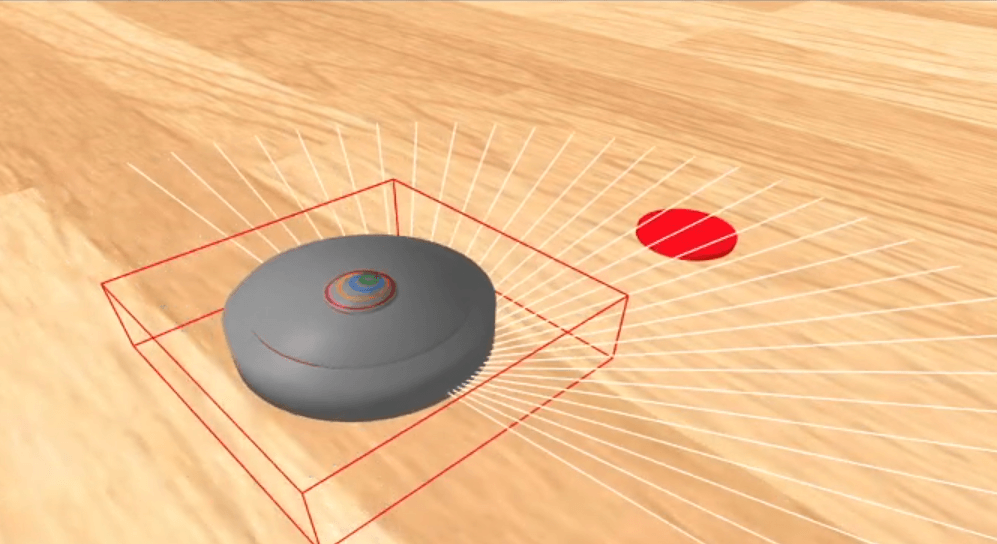
\includegraphics[width=0.8\textwidth, height=0.5\textwidth]{chapters/images/prototiporoomba.png}
    \caption{Modelos aspiradora y confeti en A-Frame}
    \label{fig:f1}
  \end{subfigure}
  \hfill
  \begin{subfigure}[b]{0.5\textwidth}
  \centering
    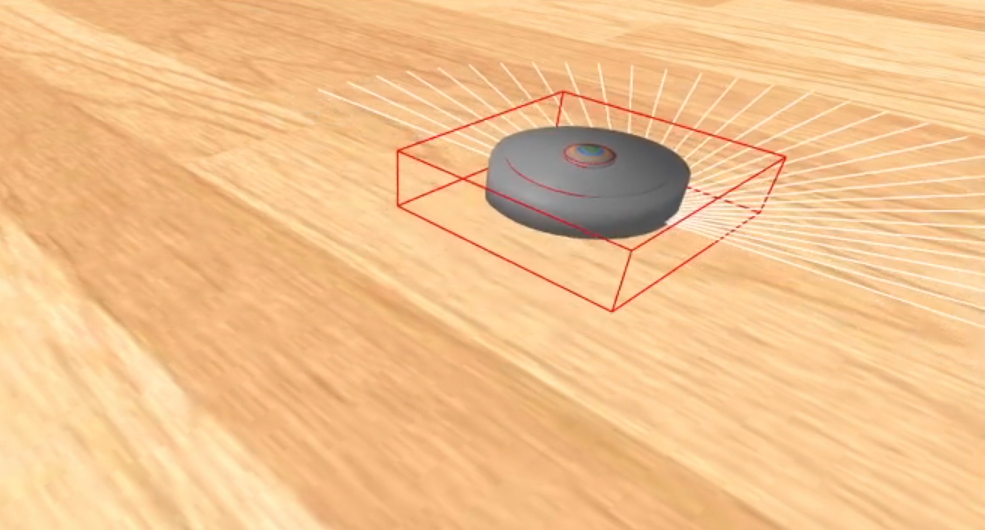
\includegraphics[width=0.8\textwidth, height=0.5\textwidth]{chapters/images/prototiporoomba2.png}
	\caption{Confeti invisible}    
    \label{fig:f2}
 
  \end{subfigure}
  \caption{Absorción por posición, el confeti es invisble cuando el robot pasa por encima.}
\end{figure}


\section{Evaluador automático}
Para contar el número de confetis que es capaz de recoger un usuario en un periodo de tiempo, se creó un evaluador automático. Este evaluador automático se introdujo dentro de la absorción, como en esa parte se calcula la distancia euclídea, ahora cada vez que d es menor o igual a 2 se suma un punto e indica que el confeti n ha sido  ``absorbido'' por el aspirador. La puntuación máxima es de 100, dado que depende del número de confetis 0-99. También se establece una cuenta atrás de 5:00 minutos. Una vez acabado el tiempo (Tiempo 00:00), aunque la aspiradora pase por encima de otros confetis visibles, éstos no serán absorbidos ni se aumentará el contador del evaluador.


En el siguiente código podemos ver todo lo necesario para la comprobación de las posiciones del confeti para la absorción y  la puntuación del evaluador. En la Figura 4.9 se muestra cómo se visualiza en la página web del ejercicio.

\begin{lstlisting}

startEvaluator = () => {
  started = true;
}
roomba=sceneEl.querySelector('#a-pibot')

 setInterval(function(){
       //console.log("Roomba",roomba.getAttribute('position').z);
      // console.log("Confeti",confeti.getAttribute('position'));
       //console.log("Confeti",confeti.getAttribute('position').z)
       for ( n = 0; n <=n_confetis ; n++) {
        d = Math.sqrt(Math.pow((array[n].z-roomba.getAttribute('position').z), 2)+Math.pow((array[n].x-roomba.getAttribute('position').x), 2));

       if ( d <= 2 ){
         num_conf="#confeti"+ String(n)
         confeti=sceneEl.querySelector(num_conf)
         if (confeti.getAttribute('visible') == true) {
	      
	      var counter= document.getElementById('time').innerHTML;
		// Tiempo: 00:00	
	      if((counter[8] =='0') && (counter[9]=='0') && (counter[11]=='0') && (counter[12]== '0')){      
		score = score;
		}else{
		score+=1;
		document.getElementById('confeti_recogido').innerHTML = "Confetti recogido: "+ score;
		}
         }
         confeti.setAttribute('visible', false);
        }
      }
	
    }, 25);
 });
\end{lstlisting}

 \begin{figure}[H]
  \centering
 
\includegraphics[width=0.35\textwidth]{chapters/images/evaluadoraspiradora.png}
  \caption{Evaluador automático para el ejercicio aspiradora robótica}
\end{figure}
\section{Solución de referencia}

Hay muchas formas diferentes  de resolver este ejercicio, en este apartado se proponen dos soluciones en los dos lenguajes que soporta Kibotics. En la Figura 4.10 se muestra una solución realizada en Scratch y en la Figura 4.11 una para Python.

\begin{figure}[H]
    \centering
    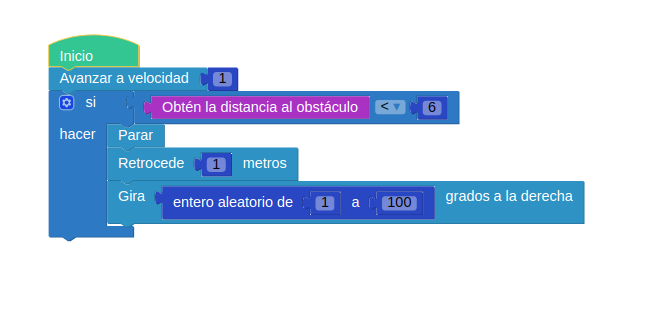
\includegraphics[width=0.7\textwidth, height=0.27\textwidth]{chapters/images/solucionroombascratch.png}
    \caption{Solución en Scratch }
    \label{fig:my_label}
\end{figure}
\begin{figure}[H]
    \centering
    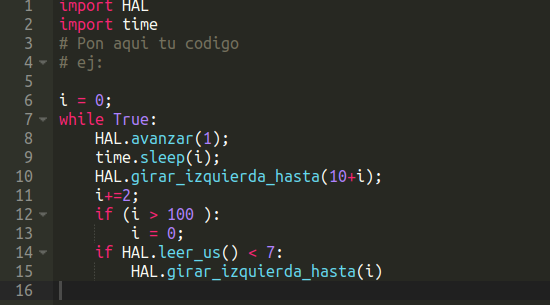
\includegraphics[width=0.7\textwidth, height=0.27\textwidth]{chapters/images/solucionroombapython.png}
    \caption{Solución en Python}
    \label{fig:my_label}
\end{figure}

En estas soluciones se ha hecho un algoritmo de cobertura usando el sensor de ultrasonidos para detectar la distancia entre el robot y los objetos de la habitación. Cuando la distancia que devuelve el sensor es muy pequeña, el robot para, retrocede y gira un número aleatorio de grados para luego continuar avanzando y aspirando por la habitación.

Este ejercicio ya está disponible en la plataforma Kibotics. También se han realizado dos vídeos promocionales para presentar el nuevo ejercicio de la plataforma con los códigos que se han mostrado en las Figuras 4.10 y 4.11. Estos vídeos \footnote{https://www.youtube.com/watch?v=5Q0TmwunYWY} \footnote{https://www.youtube.com/watch?v=Twc9wsPFjaY} sirven de ejemplo y motivación para los alumnos que vayan a realizarlo.